\section{Debug日志}
\subsection{主轨迷途衣架类Bug}
\tbc{FS长时间运行，排产结束后再排多次，几率增加。初步分析，FS调用“MU离开之前”方法比较高频，且此方法遍历站杆几乎所有的衣架。是否有其他方法，不调用此方法？}
\begin{figure}[H]%[htbp!]
	\centering
	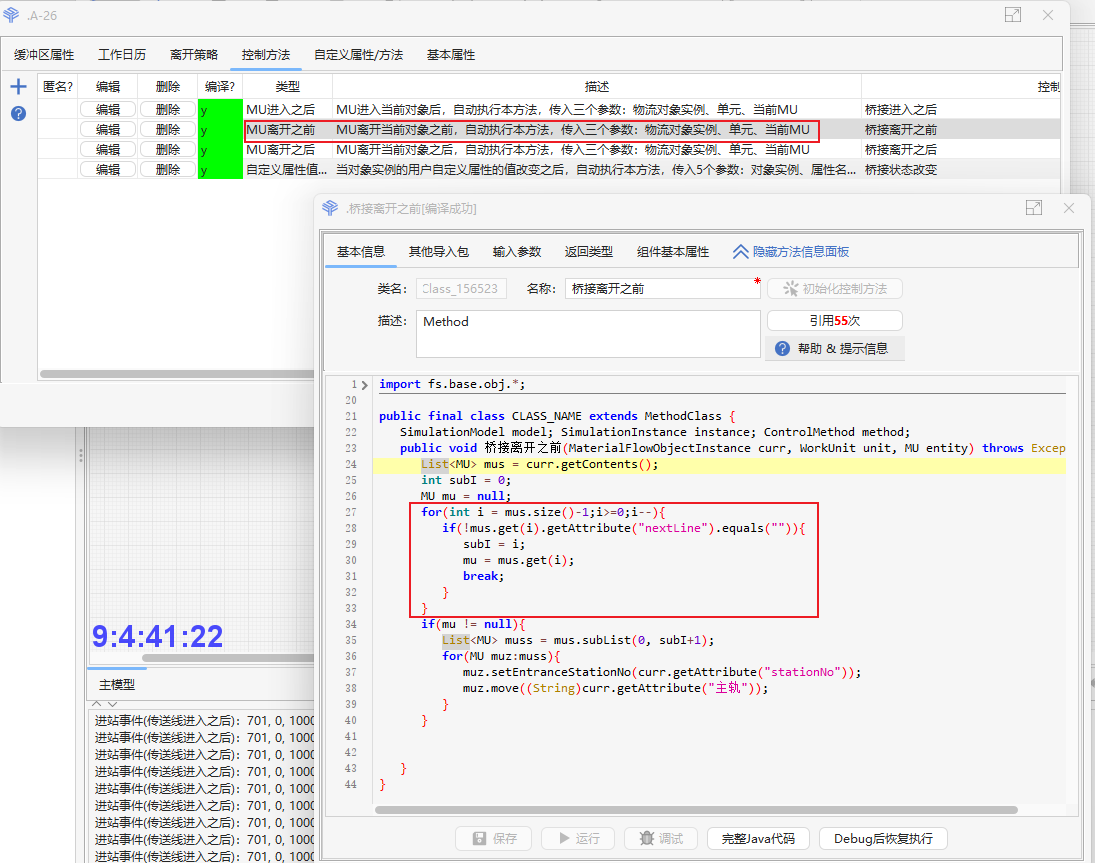
\includegraphics[width=0.8\textwidth]{pics/jack/time-consuming-method.png}
	\caption{高频调用的方法}\label{time-consuming-method}	
\end{figure}
本例使用“MU离开之前”方法调用可以简化业务逻辑，为避免高频调用，可以在方法的开头增加一个基于系统时间的判断，使得方法中的业务逻辑处理代码降低执行频率。具体实现如下：

\clearpage
\subsubsection{永久停留在通道}
	进回流通道、快速通道下发下一步指令FS没有收到。
	\begin{itemize}
		\item \it{现象}：永久停留在通道
		\item \it{数据}：查看指令日志正常，没有看到exitEvent，FS日志窗未打印对应的指令数据（UDP收到数据）
		\item \it{原因}：1）运输指令丢失，2）FS执行运输指令被其它事件覆盖属性导致指令失效
		\item \it{解决方法}：下发指令后，在Helper类中增加一个列表，入通道之后下发的指令存入列表，另设定时器检查，超过2秒没有离开通道的，重发指令。
		\begin{figure}[H]%[htbp!]
			\centering
			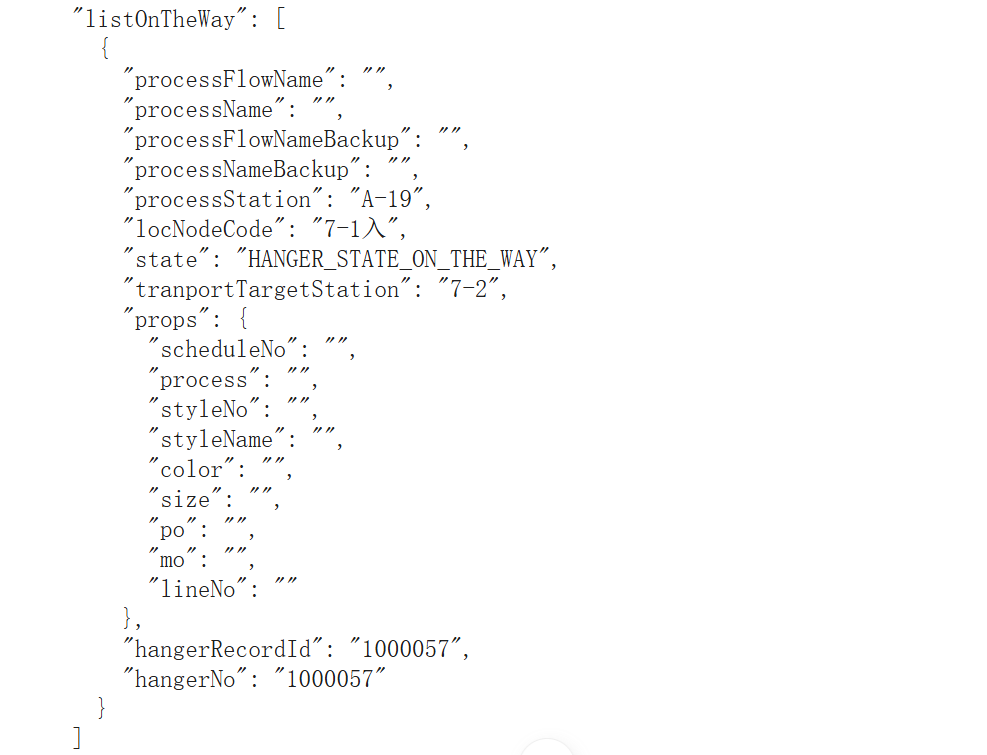
\includegraphics[width=0.6\textwidth]{pics/jack/lost-hanger-case1.png}
			\caption{迷途衣架Case1}\label{fig:lost-hanger-case1}	
		\end{figure}
		\begin{enumerate}[label=\alph*)]
			\item \bf{使用哈希表}：Map<String, TimeAndCommand> commandMap，其中的 TimeAndCommand 定义如下：
			\begin{lstlisting}
    @Data
    static class TimeAndCommand {
        /** 指令发送时间 */
        private long time;
        /** 指令字符串 */
        private String cmdJsonString;
        public TimeAndCommand(long tm, String cmd) {
            time = tm;
            cmdJsonString = cmd;
        }
    }
			\end{lstlisting}
			\item \bf{put}：衣架进入快速通道/回流通道，下发下一步运输指令时，以 hangerId 为 key
			\item \bf{remove}：衣架出杆时，从 commandMap 中移除 key 为衣架的元素
			\item \bf{update}：衣架更改目的地，刚好在 commandMap 中，更新元素
			\item \bf{timed task}：每 1 秒检查一次 commandMap，滞留超过 2 秒的衣架，重复发送指令

		\end{enumerate}
	\end{itemize}
\clearpage
\subsubsection{衣架在主轨绕圈}
	进回流通道、快速通道下发下一步指令过快，FS的进站处理函数覆盖了下一站数据 
	\begin{itemize}
		\item \it{现象}：在主轨绕圈
		\item \it{数据}：查看指令、事件日志，可看到如下数据：
		\begin{figure}[H]%[htbp!]
			\centering
			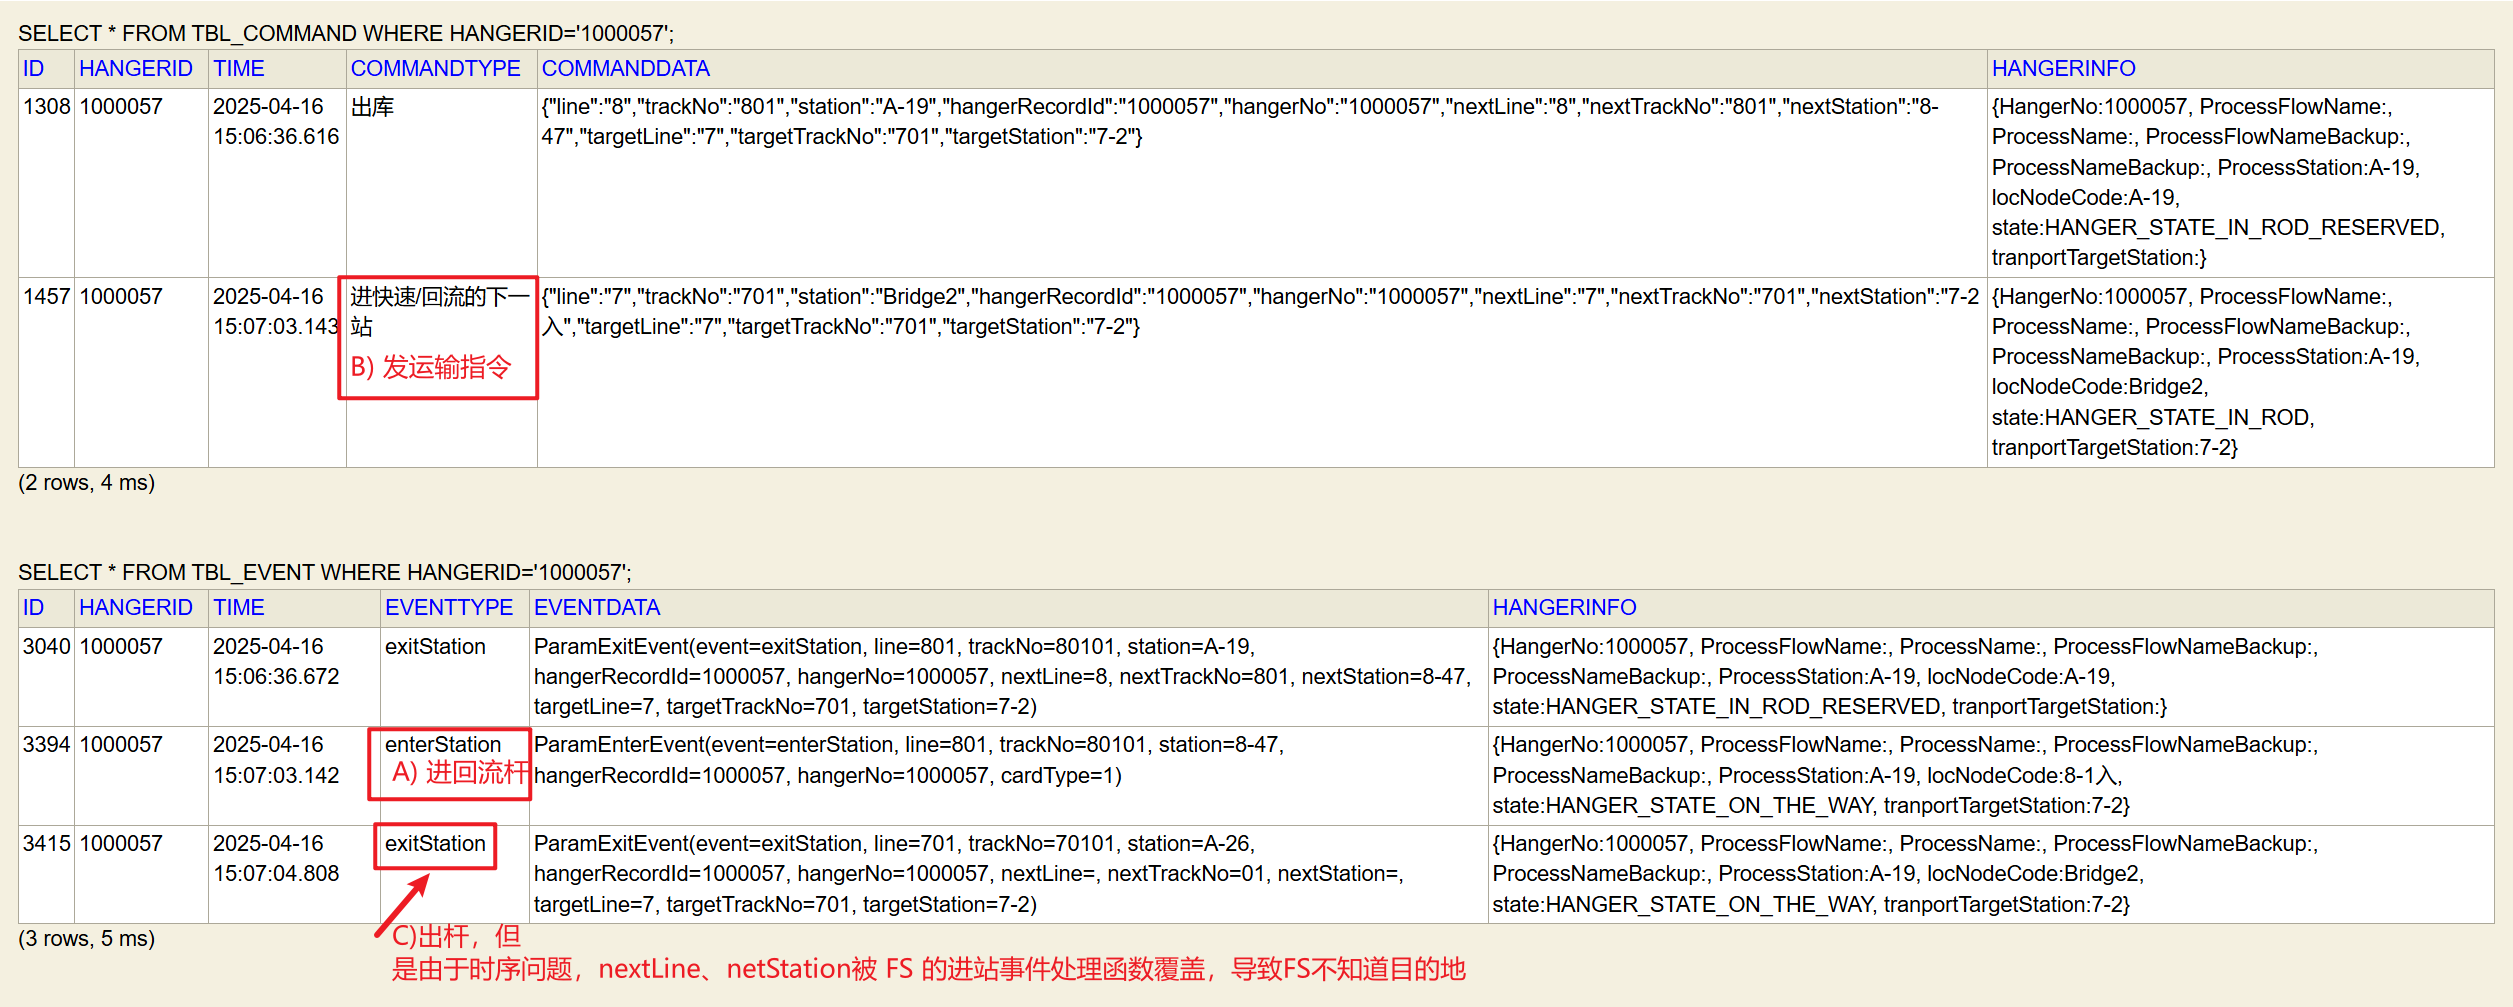
\includegraphics[width=0.7\textwidth]{pics/jack/lost-hanger-case2.png}
			\caption{迷途衣架Case2}\label{fig:lost-hanger-case2}	
		\end{figure}
		\item \it{原因}：进回流通道、快速通道下发下一步指令过快，FS的进站处理函数覆盖了下一站数据。
		\item \it{解决方法}：1）FS“传送线进入之后”ControlMethod中计数，超过2次，就重新发送指令。下图中没有发送这个事件（实际的吊挂系统下位机系统不发这个事件，此方法只在虚拟调试时使用）。2）延迟发送下一步运输指令，问题缓解，但不能彻底解决。
		\begin{figure}[H]%[htbp!]
			\centering
			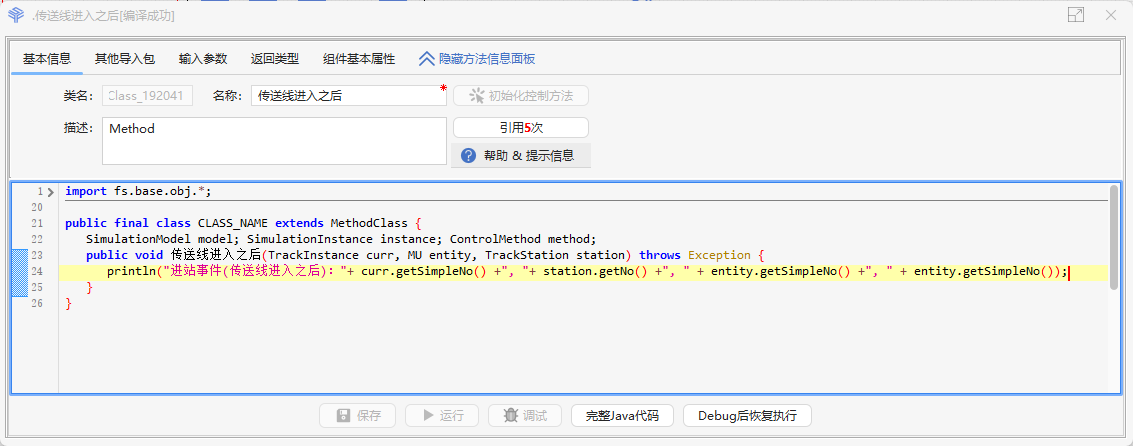
\includegraphics[width=0.7\textwidth]{pics/jack/enter-track.png}
			\caption{进传送线事件（包括正常的TrackStation和特殊的TrackStation 0）}\label{fig:enter-track}
		\end{figure}
	\end{itemize}
\clearpage
\subsubsection{已叫料的衣架不出库}
	\begin{figure}[H]%[htbp!]
		\centering
		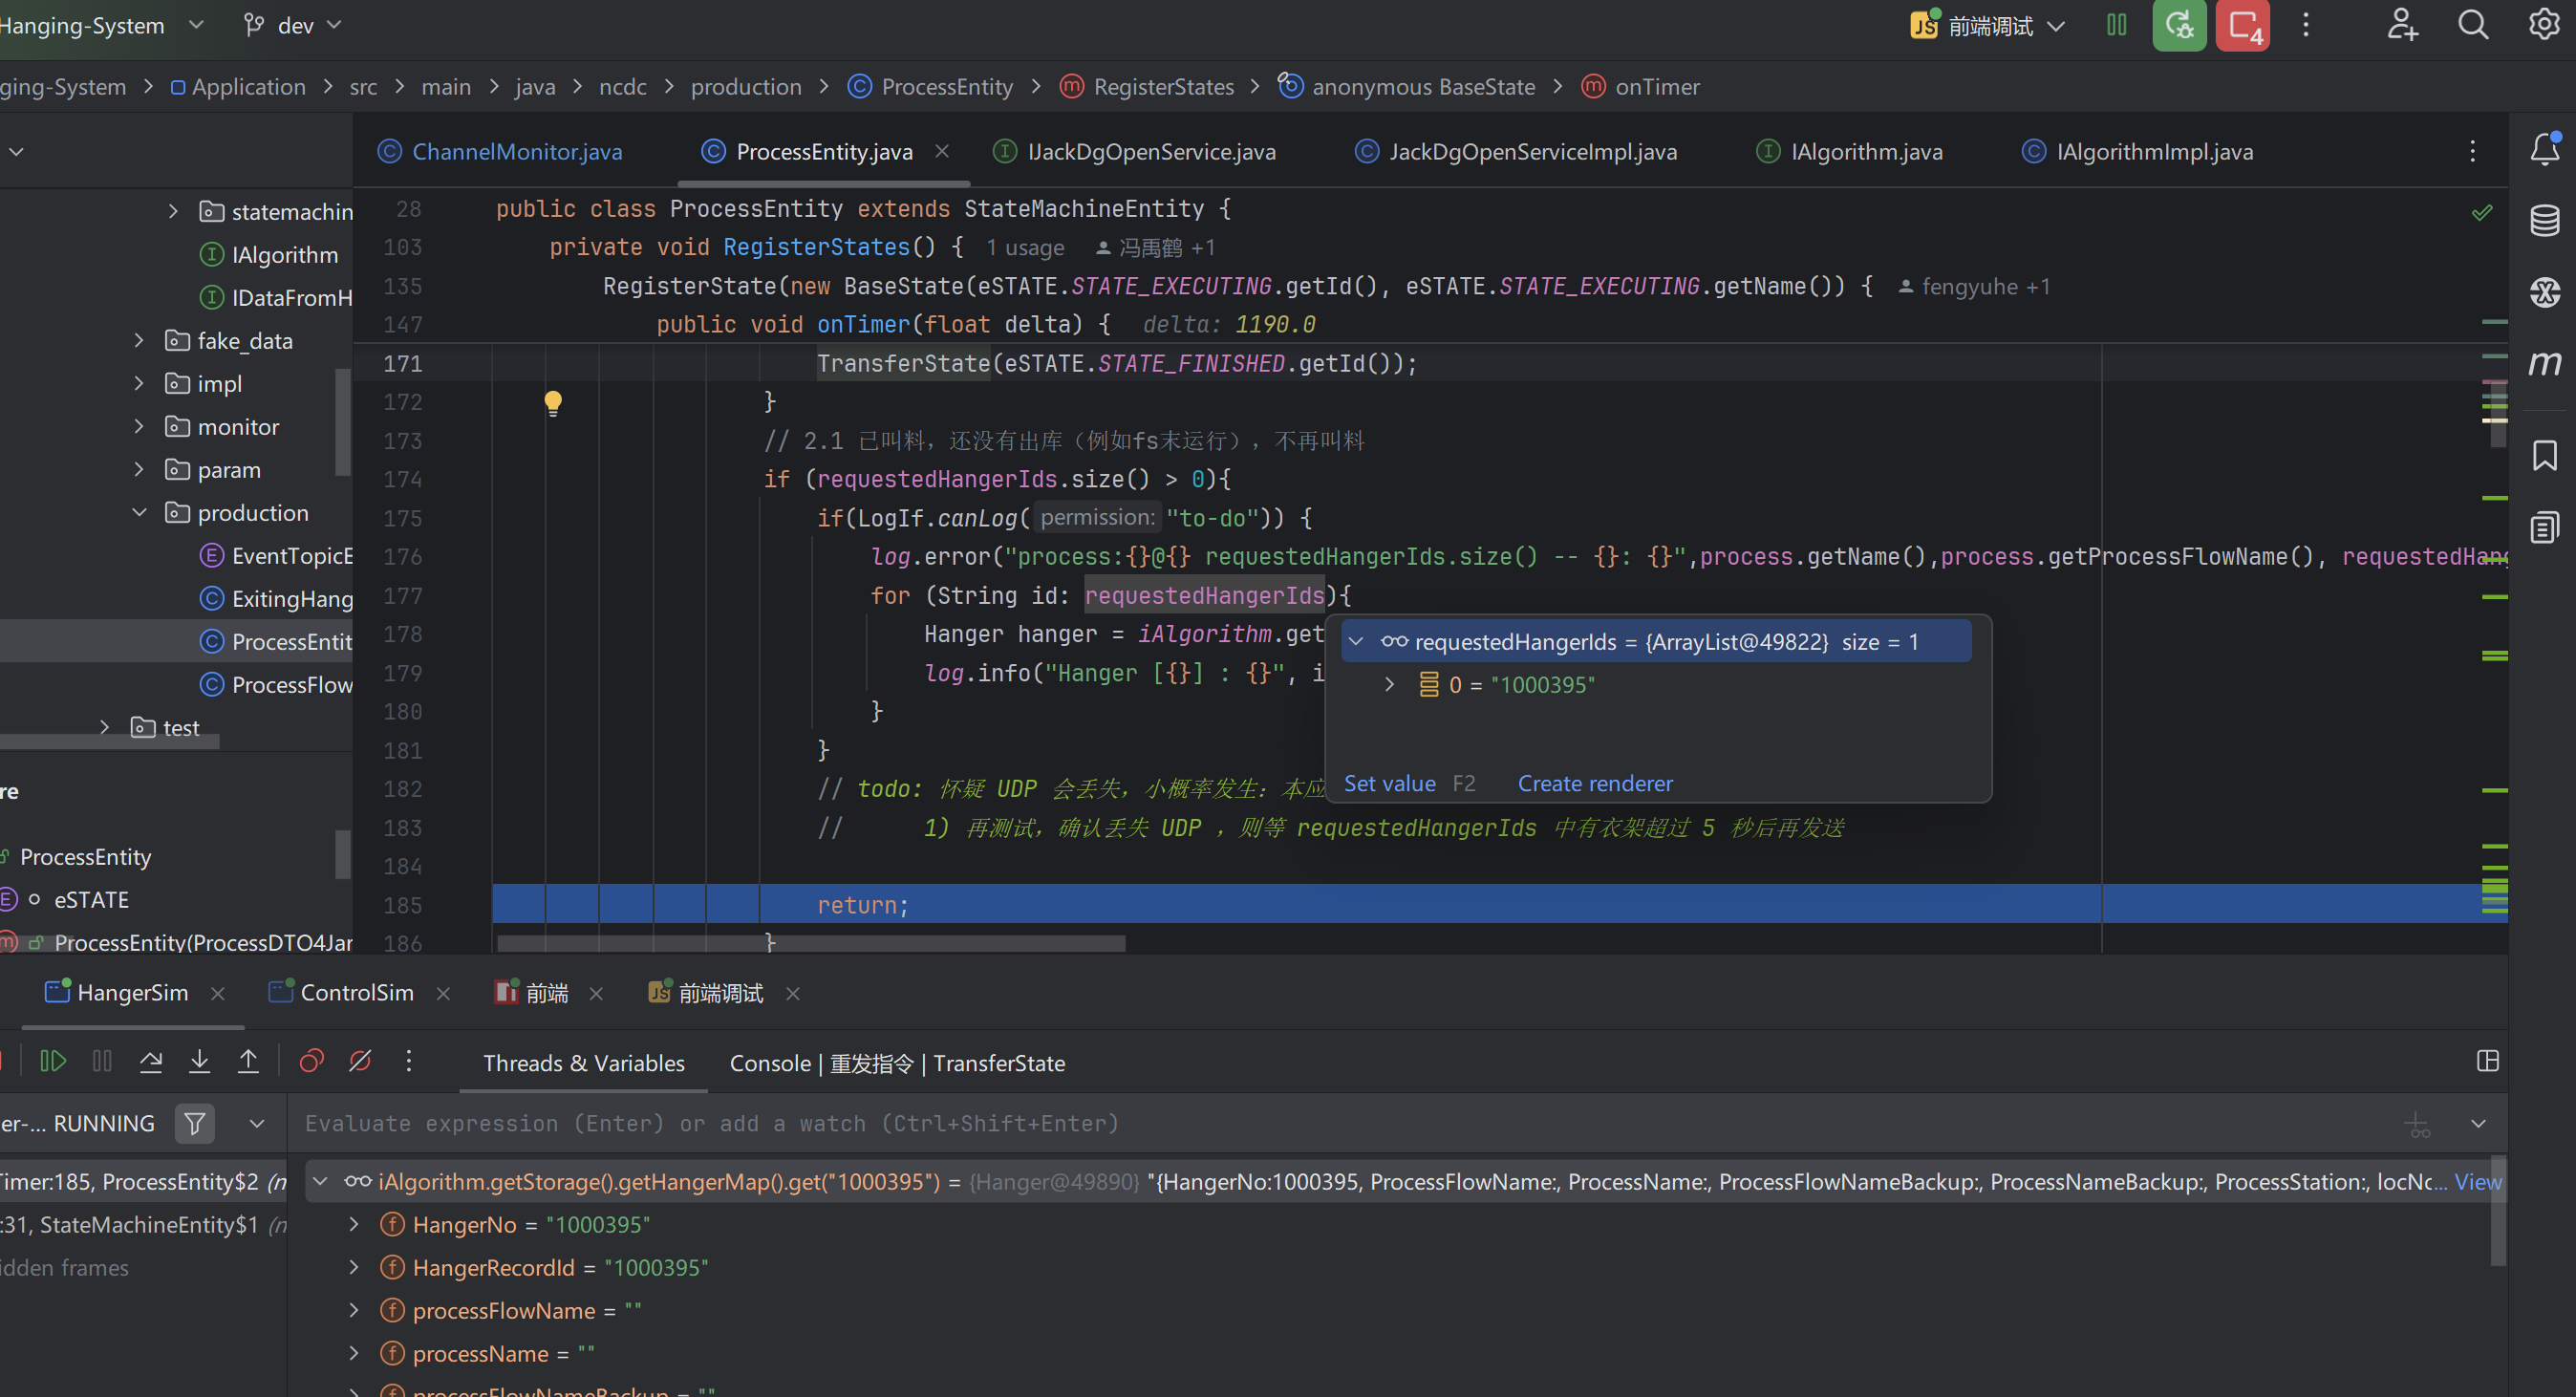
\includegraphics[width=0.95\textwidth]{pics/jack/lost-hanger-case3.png}
		\caption{衣架不出库的原因，迷途衣架Case3}\label{fig:lost-hanger-case3}
	\end{figure}
	\begin{itemize}
		\item \it{现象}：衣架不出库，例如挂片工序没有完成任务，也没有再叫料。
		\item \it{原因}：如图\ref{fig:lost-hanger-case3}所示，\it{requestedHangerIds}不为空，且不会再清空。导致这个问题的原因，是FS没有发出站事件。
		\item \it{解决方法}: 将\it{requestedHangerIds}改造为Map<String, Long>，key为衣架ID，value为时间戳。上图判断requestedHangerIds是否为空的处理逻辑，加上是否超时的判断，未超时继续等，超时则取消 hanger的预订标识，并从\it{requestedHangerIds}中移除。
	\end{itemize}


\clearpage
\subsection{意外混存类Bug}
\begin{enumerate}[label=\arabic*)]
\item \bf{满光电重入库，所选库位已经有在途衣架}
	\begin{figure}[H]%[htbp!]
		\centering
		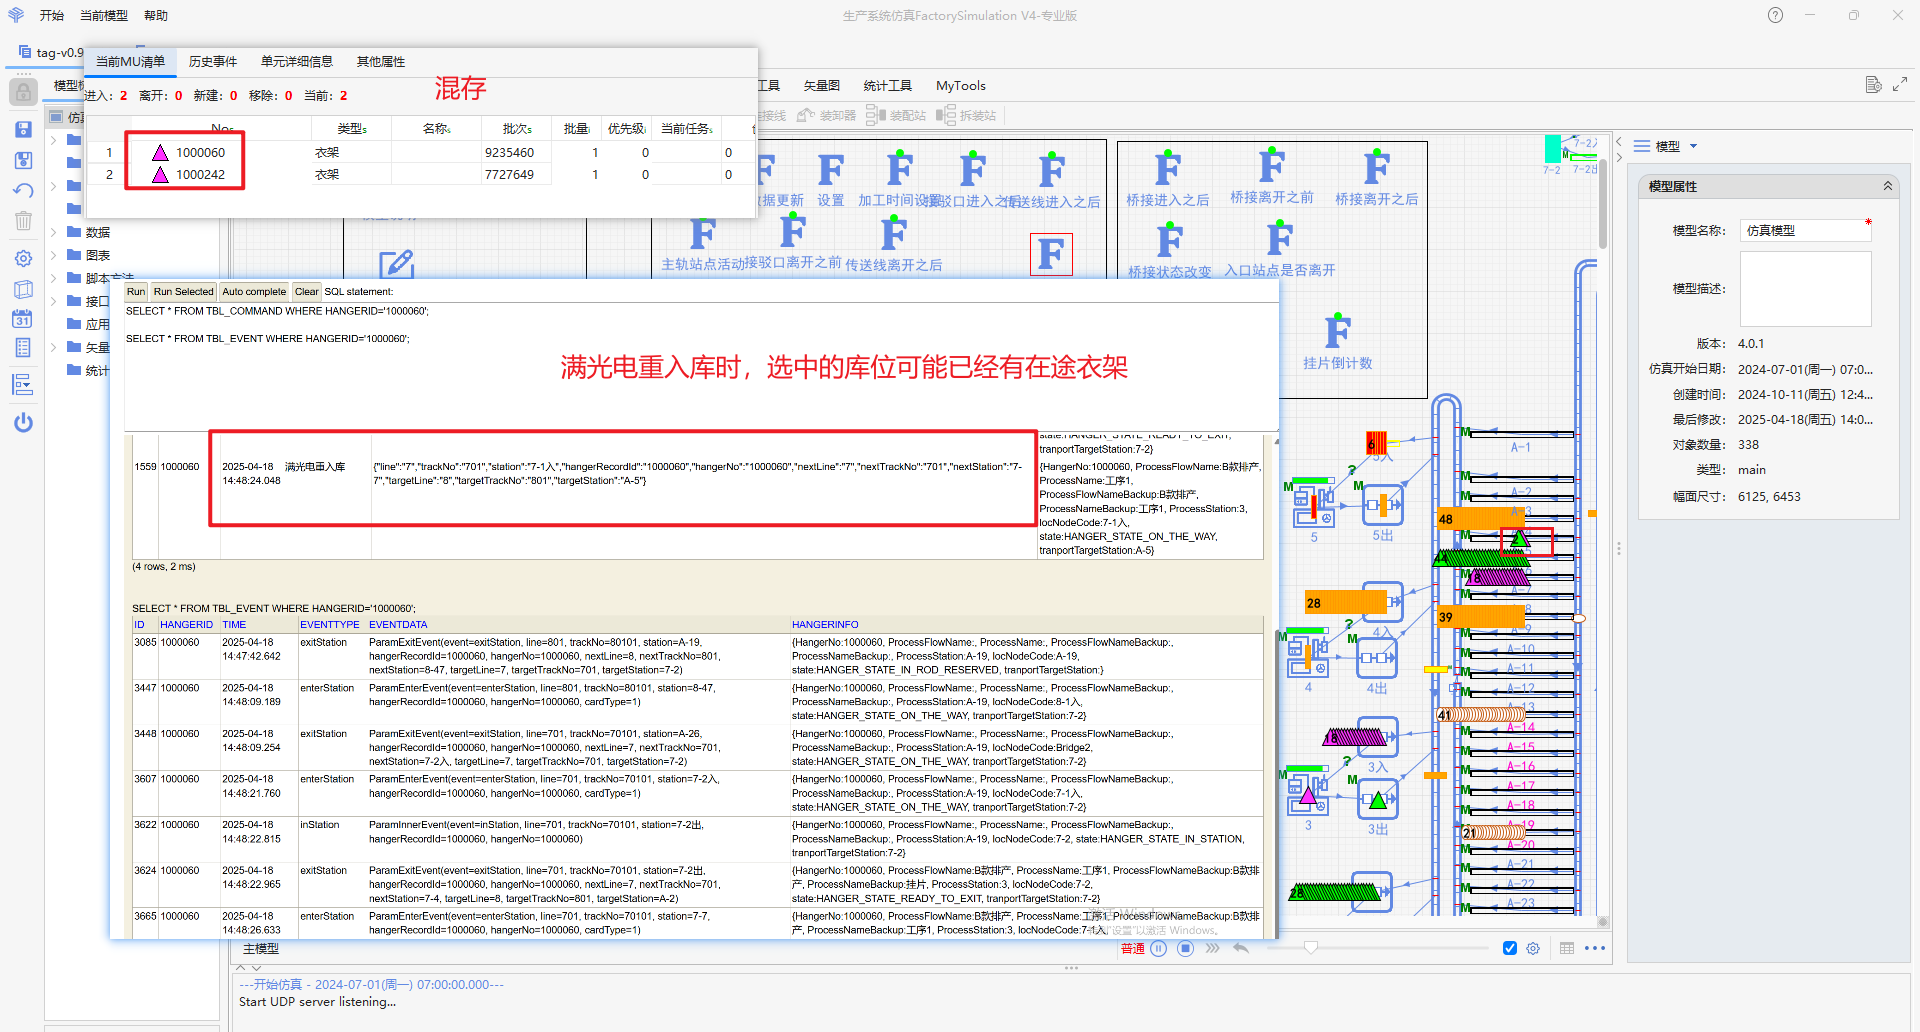
\includegraphics[width=0.9\textwidth]{pics/jack/mix-bug1.png}
		\caption{意外混存 Case 1}\label{fig:mix-bug1}
	\end{figure}

\end{enumerate}